\selectlanguage{ngerman}%
\frenchspacing%
\begin{ledgroupsized}[r]{120mm}%
\footnotesize%
\pstart%
\noindent%
\textbf{Überlieferung:}%
\pend%
\end{ledgroupsized}%
\begin{ledgroupsized}[r]{114mm}%
\footnotesize%
\pstart%
\parindent -6mm%
\makebox[6mm][l]{\textit{L}}%
Aufzeichnung:
LH\;XXXVII\;3, Bl.\;115--116.
Ein Bogen 4\textsuperscript{o};
\href{\Scan{LH_37_03_115-116wz}}{Wasserzeichen} mittig.
Vier ganzseitig beschriebene Seiten.
\pend%
\end{ledgroupsized}%
\vspace{5mm}%
\begin{ledgroup}%
\footnotesize%
\pstart%
\noindent%
\textbf{Datierungsgründe:}
Die Datierung der Aufzeichnung N.\;\ref{60205} beruht auf äußeren Eigenschaften des Text\-trägers %
sowie auf inhaltlichen Betrachtungen.
Siehe die ausführliche Begründung auf S.~\pageref{60205_dat}.%
\pend%
\end{ledgroup}%
\selectlanguage{latin}%
\frenchspacing%
\vspace{8mm}%
\normalsize%
\pstart%
\noindent%
\lbrack%
\href{\Scan{LH_37_03_115r}}%
{115\,r\textsuperscript{o}%
}%
\rbrack%
\hfill%
De nova pressione aeris%
\indexS{pressio aeris}
subtilioris%
\indexS{aer subtilior}%
\hfill%
\phantom{\lbrack115\,r\textsuperscript{o}\rbrack}%
\pend%
\pstart%
\centering%
etiam intra locum aere communi exhaustum%
\indexS{locus exhaustus aere}
deprehensa,
\pend%
\pstart%
\centering%
et in aere libero%
\indexS{aer liber}
pressionem a cylindro aeris crassi ortam%
\indexS{pressio orta a cylindro aeris}%
\indexS{cylinder aeris}%
\indexS{aer crassus}
longe superante%
\pend%
\vspace{0.5em}%
\pstart%
\noindent%
\edlabel{LH_37_03_115-116_115r_veteres-1}%
\edtext{%
}{%
\xxref{LH_37_03_115-116_115r_veteres-1}{LH_37_03_115-116_115r_veteres-2}%
\lemma{Veteres \lbrack...\rbrack\ abhorreat}%
\Cfootnote{%
Nicht ermittelt.%
}}%
Veteres%
\indexS{veteres}
cum observarent
aquam ex vase pleno%
\indexS{vas plenum aqua}
angusti oris%
\indexS{os vasis angustum}
non
effluere %
\indexS{aqua non effluens e vase}
nisi alio
\edtext{%
adhuc%
}{%
\lemma{adhuc}%
\Bfootnote{%
\textit{erg.\:L}%
}}
foramine aperto,%
\indexS{foramen apertum in vase}
eandem in
\edtext{%
antlia aspirante%
\indexS{antlia aspirans}
sequi embolum ascendentem,%
\indexS{embolus ascendens in antlia}%
\indexS{aqua sequens embolum ascendentem}
follem quoque foramine carentem%
\indexS{follis carens foramine}%
}{%
\lemma{antlia}%
\Bfootnote{%
\textit{(1)}~sequi em %
\textit{(2)}~aspirante sequi embolum ascendentem, %
\textit{(a)}~\bars{item \textit{erg.}} %
\textit{(b)}~follem %
\bars{quoque \textit{erg.}} foramine carentem%
~\textit{L}%
}}
magna licet vi adhibita%
\indexS{vis adhibita}
non posse
\edtext{%
aperiri,
id ajebant fieri%
}{%
\lemma{aperiri,}%
\Bfootnote{%
\textit{(1)}~ventosam chirurgicam calefacto citius aere uti applicatam %
\textit{(2)}~id ajebant fieri%
~\textit{L}%
}%
}
ob fugam vacui,%
\indexS{fuga vacui}
quod natura%
\indexS{natura abhorrens vacuum}
abhorreat.%
\edlabel{LH_37_03_115-116_115r_veteres-2}
Nam embolo ascendente
si aqua non sequeretur,
\edtext{%
mansur\lbrack u\rbrack m%
}{%
\lemma{mansuram}%
\Bfootnote{%
\textit{L\;ändert Hrsg.}%
}}
intra embolum%
\indexS{embolus ascendens in antlia}
et aquam%
\indexS{aqua sequens embolum ascendentem}
locum vacuum.%
\indexS{locus vacuus aere}
Sed
\edtext{%
Galilaeus%
\indexN{\textls{Galilei} (Galilaeus, Galileus), Galileo 1564\textendash1642}
didicit ab
\edtext{%
Hydraulis%
\indexS{hydraulum}
hanc%
}{%
\lemma{Hydraulis}%
\Bfootnote{%
\bars{Italis \textit{gestr.}} hanc%
~\textit{L}%
}}
naturae resistentiam%
\indexS{resistentia naturae}%
\indexS{natura abhorrens vacuum}
posse
\edtext{%
vinci a pondere aquae%
}{%
\lemma{vinci}%
\Bfootnote{%
\textit{(1)}~per aquam %
\textit{(2)}~a pondere aquae%
~\textit{L}%
}}
altitudinis circiter 35 pedum,%
\indexS{pondus aquae 35 pedum}%
\indexS{pes}
sive aquam in antliis aspirantibus%
\indexS{antlia aspirans}
ultra hanc altitudinem%
\indexS{altitudo 35 pedum}
elevari non posse,%
\indexS{aqua elevata in antlia}%
}{%
\lemma{Galilaeus \lbrack...\rbrack\ posse}%
\Cfootnote{%
Siehe
G.\;\textsc{Galilei},
\textit{Discorsi}, giornata I
(Leiden 1638,\cite{00050}
S.\;17;
\textit{GO} VIII,\cite{00048}
S.\;63.36--64.25).
}}
quod etiam in fodinis%
\indexS{fodina}
\edtext{%
dudum%
}{%
\lemma{dudum}%
\Bfootnote{%
\textit{erg.\:L}%
}}
experti
\edtext{%
sunt nostri.%
}{%
\lemma{sunt}%
\Bfootnote{%
\textit{(1)}~Germani.\indexS{Germanus} %
\textit{(2)}~nostri.%
~\textit{L}%
}}
Postea
\edlabel{LH_37_03_115-116_115_torricelli-1}%
\edtext{}{%
\xxref{LH_37_03_115-116_115_torricelli-1}{LH_37_03_115-116_115_torricelli-2}%
\lemma{Torricellius \lbrack...\rbrack\ tegerent}%
\Cfootnote{%
Siehe \textsc{E.\;Torricelli},
Brief an M.\;Ricci vom 11.\;Juni 1644\cite{00107}
(C.\,\textsc{Dati},
\textit{Lettera a Filaleti ... della famosissima esperienza dell’argento vivo},
Florenz 1663, S.\;20\,f.;\cite{00032}
\textit{TO}\;III, S.\;186--188).\cite{00108}%
}}%
Torricellius%
\indexN{\textls{Torricelli} (Torricellius), Evangelista 1608\textendash1647}
pro pondere 35 pedum aquae%
\indexS{pondus aquae 35 pedum}%
\indexS{pes}
invenit pondus 27
\edtext{%
pollicum Hydrargyri,%
\indexS{pondus hydrargyri 27 pollicum}%
\indexS{hydrargyrum}%
\indexS{pollex}%
}{%
\lemma{pollicum}%
\Bfootnote{%
\textit{(1)}~Mercurii\indexS{mercurius} %
\textit{(2)}~Hydrargyri%
~\textit{L}%
}}
cujus altitudo%
\indexS{altitudo 27 pollicum}
tanto minor sufficit,
quanto ipsum est aqua
\edtext{%
ponderosius.
Nam tubum%
\indexS{tubus Torricellianus}
qui unum foramen%
\indexS{foramen tubi}
apertum habebat%
\lbrack,\rbrack\
Hydrargyro%
\indexS{hydrargyrum}%
\indexS{tubus impletus hydrargyro}
implevit %
et invertit,
quo facto expertus est
non obstante fuga vacui%
\indexS{fuga vacui}%
\bracks{,}
ex tubo effluere Mercurium%
\indexS{mercurius effluens e tubo Torricelliano}
exceptis 27 pollicibus %
qui in tubo suspensi manent%
\indexS{mercurius suspensus in tubo Torricelliano}%
\bracks{,}
locum supra se vacuum%
\indexS{locus vacuus aere}
\bracks{(}%
quantum sensu judicari potest%
\indexS{sensus}%
\indexS{judicium sensus}%
\bracks{)}
relinquentes.
Unde%
}{%
\lemma{ponderosius.}%
\Bfootnote{%
\bars{Nam tubum
\textit{(1)}~unum tantum apertum habentem %
\textit{(2)}~qui unum %
\lbrack...\rbrack\ expertus est %
\textit{(a)}~Mercurium effluere ex tubo non obstante fuga vacui %
\textit{(b)}~non obstante %
\lbrack...\rbrack\ qui in 
\textit{(aa)}~eo %
\textit{(bb)}~tubo suspensi %
\lbrack...\rbrack\ se vacuum %
\textit{(aaa)}~relinquentes %
\textit{(bbb)}~quantum sensu judicari potest relinquentes %
\textit{erg.}} %
\textit{(1)}~Cumque inde a %
\textit{(2)}~Unde%
~\textit{L}%
}}
judicavit Torricellius%
\indexN{\textls{Torricelli} (Torricellius), Evangelista 1608\textendash1647}
pondus aeris externi circumfusi%
\indexS{pondus aeris externi}%
\indexS{aer externus}%
\indexS{aer circumfusus}
et in locum aere vacuum%
\indexS{locus vacuus aere}
tota sua vi intrare%
\indexS{vis aeris intrantis in locum vacuum}
\edtext{%
intent\lbrack i\rbrack%
}{%
\lemma{intentis}%
\Bfootnote{%
\textit{L\;ändert Hrsg.}%
}}
causam esse
\edtext{%
difficultatis%
\indexS{difficultas in embolis extrahendis}
quae sentitur%
}{%
\lemma{difficultatis quae}%
\Bfootnote{%
\textit{(1)}~scitur %
\textit{(2)}~sentitur%
~\textit{L}%
}}
in embolis extrahendis,%
\indexS{embolus extrahendus}
et exaltationis aquae%
\indexS{exaltatio aquae}%
\indexS{aqua exaltata}
\edtext{%
quippe%
}{%
\lemma{quippe}%
\Bfootnote{%
\textit{erg.\:L}%
}}
quae non tam attrahitur %
\indexS{aqua attracta}
quam ab aere incumbente%
\indexS{aer incumbens telluri}
\edtext{%
sursum exprimitur.%
\indexS{aqua expressa ab aere incumbente}
Et pondus aeris%
\indexS{pondus aeris}
telluri%
\indexS{tellus}
incumbentis%
\indexS{aer incumbens}
tantum esse circiter
quantum esset pondus aquae,%
\indexS{pondus aquae 35 pedum}
si 35 ejus pedes
aut 27 pollices Hydrargyri%
\indexS{pondus hydrargyri 27 pollicum}
globum telluris%
\indexS{globus telluris}%
\indexS{tellus}
tegerent.%
\edlabel{LH_37_03_115-116_115_torricelli-2}%
}{%
\lemma{sursum}%
\Bfootnote{%
\textit{(1)}~premitur. %
\textit{(2)}~exprimitur. Et %
\textit{(a)}~hoc pondus aeris aequ %
\textit{(b)}~pondus aeris telluri incumbentis %
\textit{(aa)}~aequari circiter ponderi 35 
\textit{(bb)}~tantum esse %
\lbrack...\rbrack\ esset pondus %
\textit{(aaa)}~aquae, si 35 ejus pedes superficiem globi telluris %
\textit{(bbb)}~, si 35 pedes aquae aut %
\textit{(aaaa)}~\textlangle\textendash\textrangle\ %
\textit{(bbbb)}~Hydrargyrii aut %
\textit{(ccc)}~aquae, si %
\lbrack...\rbrack\ telluris tegerent.%
~\textit{L}%
}}
\edlabel{LH_37_03_115-116_115r_pascal-1}%
\edtext{}{%
\xxref{LH_37_03_115-116_115r_pascal-1}{LH_37_03_115-116_115r_pascal-2}%
\lemma{Cumque \lbrack...\rbrack\ deprehendit}%
\Cfootnote{%
Siehe %
B.\;\textsc{Pascal},
\textit{Récit de la grande expérience}, 1648\cite{02577} %
(\textit{Traitez}, Paris 1663, S.\;165--194;\cite{00081}
\textit{PO}\;II, S.\;653--690).\cite{01524}
Leibniz hatte 1672 die \textit{Traitez} gelesen und exzerpiert;
vgl. \textit{LSB} VIII,\;1 N.\;38.\cite{01038}%
}}%
Cumque hinc sequeretur
in altissimis montibus%
\indexS{mons altissimus}
minorem debere esse altitudinem Mercurii
in tubo
\edtext{%
Torricellian\lbrack o\rbrack%
\indexS{tubus Torricellianus}%
}{%
\lemma{Torricelliani}%
\Bfootnote{%
\textit{L\;ändert Hrsg.}%
}}
suspensi,%
\indexS{altitudo mercurii suspensi}%
\indexS{mercurius suspensus in tubo}
\edtext{%
quia aeris infra montem positi pondus%
\indexS{aer positus infra montem}%
\indexS{pondus aeris detrahendum}
detrahendum est,%
}{%
\lemma{quia}%
\Bfootnote{%
\textit{(1)}~aer infra montem positus eum %
\textit{(2)}~aeris infra %
\lbrack...\rbrack\ detrahendum est, %
\textit{erg.\:L}%
}}
hoc expertus Pascalius%
\indexN{\textls{Pascal} (Pascalius), Blaise 1623\textendash1662}
verum deprehendit.%
\edlabel{LH_37_03_115-116_115r_pascal-2}
Et jam
\edlabel{LH_37_03_115-116_115r_pascal-3}%
\edtext{}{%
\xxref{LH_37_03_115-116_115r_pascal-3}{LH_37_03_115-116_115r_pascal-4}%
\lemma{pro indubitato \lbrack...\rbrack\ avellendae}%
\Cfootnote{%
Siehe \textsc{Pascal},
\textit{De la pesanteur de la masse de l'air},
cap.\;3\cite{01432}
(\textit{Traitez}, S.\;95\,f.;\cite{00081}
\textit{PO}\;II, S.\;1082\,f.).\cite{01524}%
}}%
pro indubitato habuit,
\edtext{%
praecise aperiri posse follem clausum,%
\indexS{follis clausus}
aut divelli posse duas tabulas politas
sibi impositas,%
\indexS{tabulae politae impositae sibi}
pondere
quod aequivaleat cylindro altitudinis 35 pedum aquae,%
\indexS{pondus cylindri aquae 35 pedum}%
\indexS{cylinder aquae 35 pedum}%
\indexS{altitudo 35 pedum}
basis vero seu crassitiei tantae
quanta est latitudo follis,%
\indexS{follis clausus}
aut tabulae minoris avellendae.%
\indexS{tabula polita avellenda}%
\indexS{avulsio tabularum politarum}%
\edlabel{LH_37_03_115-116_115r_pascal-4}%
}{%
\lemma{praecise}%
\Bfootnote{%
\textit{(1)}~pondere 35 pedum aquae basin latitudini follis aut minimae ex duabus t %
\textit{(2)}~pond %
\textit{(3)}~aperiri posse follem clausum, aut %
\textit{(a)}~distrahi posse %
\textit{(b)}~divelli posse %
\lbrack...\rbrack\ impositas, pondere %
\textit{(aa)}~cylindr %
\textit{(bb)}~quod aequivaleat cylindro %
\bars{altitudinis \textit{erg.}} 35 pedum %
\lbrack...\rbrack\ minoris avellendae.%
~\textit{L}%
}}
\pend%
\pstart%
\edlabel{LH_37_03_115-116_115_lpo-1}%
Verum haec
licet pulchre conclusa viderentur,
turbarunt Experimenta posteriora%
\indexS{experimentum turbans}%
\lbrack;\rbrack\
nam
\edlabel{LH_37_03_115-116_115r_Brouncker-1}%
\edtext{}{%
\xxref{LH_37_03_115-116_115r_Brouncker-1}{LH_37_03_115-116_115r_Brouncker-2}%
\lemma{Brounckerus \lbrack...\rbrack\ altitudine}%
\Cfootnote{%
Hierüber berichtet
\textsc{J.\;Wallis}, \textit{Mechanica}, cap.\;XIV, prop.\;13, schol.
(London 1670--1671, Bd.\;II, S.\;740;\cite{00301}
\textit{WO}~I, S.\;1051);\cite{01008}
Leibniz hatte 1674--1675 die Stelle exzerpiert;
vgl. \textit{LSB} VIII,\;2 N.\;8, S.\;96.18--97.6.%
\cite{01343}
Siehe zudem
J.\;\textsc{Wallis}, "An Extract of letters"
(\textit{PT} VII, 1672, S.\;5160).\cite{00213}%
}}%
\edtext{%
Brounckerus%
\indexN{\textls{Brouncker} (Brunckerus), William Viscount 1620\textendash1684}
observavit%
}{%
\lemma{Brounckerus}%
\Bfootnote{%
\bars{in Anglia \textit{gestr.}} observavit%
~\textit{L}%
}}
aliquando
Mercurium ab aere jam purgatum%
\indexS{mercurius purgatus aere}
ad 70 et ultra pollices%
\indexS{pollex}
in aere libero%
\indexS{aer liber}
suspensum%
\indexS{mercurius suspensus ad 70 pollices}
mansisse,
\edtext{%
leviter tamen concusso tubo%
\indexS{tubus concussus}
facile decidisse
remanente tantum communi 27 pollicum altitudine.%
\indexS{altitudo mercurii 27 pollicum}%
\indexS{pollex}%
}{%
\lemma{leviter tamen \lbrack...\rbrack\ pollicum altitudine}%
\Bfootnote{%
\textit{erg.\:L}%
}}%
\edlabel{LH_37_03_115-116_115r_Brouncker-2}
\edlabel{LH_37_03_115-116_115r_Hugenius-1}%
\edtext{}{%
\xxref{LH_37_03_115-116_115r_Hugenius-1}{LH_37_03_115-116_115r_Hugenius-2}%
\lemma{Hugenius \lbrack...\rbrack\ cesset}%
\Cfootnote{%
Siehe
\textsc{C.\;Huygens}, "Extrait d'une lettre"
(\textit{JS}, 25.\;Juli 1672, S.\;140;\cite{00062}
\textit{HO} VII, S.\;206).\cite{00113}
Mit diesem Aufsatz hatte sich Leibniz 1672--1673 ausführlich auseinandergesetzt;
vgl. insbesondere
\textit{LSB} VIII,\:1 N.\;39.%
\cite{01069}%
}}%
Hugenius%
\indexN{\textls{Huygens} (Hugenius, Ugenius, Hugens, Huguens), Christiaan 1629\textendash1695}
quoque
\edtext{%
notavit,
quod aqua%
\indexS{aqua purgata aere}
aere purgata%
}{%
\lemma{notavit,}%
\Bfootnote{%
\textit{(1)}~aquam %
\textit{(2)}~quod aqua %
\bars{aere purgata \textit{erg.}}%
\textit{L}%
}}
ex vase exhauriri possit%
\indexS{aqua exhausta e vase}%
\indexS{vas plenum aqua}
ope Siphonis inversi bicruri,%
\indexS{sipho bicrurus}
licet durante effluxu%
\indexS{effluxus aquae e vase}
aer ex
\edtext{%
\edlabel{LH_37_03_115-116_115r_dfe-1}%
Recipiente Magdeburgico%
\indexS{recipiens Magdeburgicus}%
\edlabel{LH_37_03_115-116_115r_dfe-2}%
}{%
\lemma{Recipiente Magdeburgico}%
\Cfootnote{%
Pneumatische Vorrichtung zur Vakuumerzeugung.
Leibniz spielt auf die Instrumente an,
die in \textsc{O.\,v.\,Guericke},
\textit{Experimenta nova}, l.\;III
(Amsterdam 1672, S.\;71--124)\cite{00055}
geschildert sind.
Hieraus hatte er 1672 Exzerpte angefertigt;
vgl. \textit{LSB} VIII,\;1 N.\;36.\cite{01197}%
}}
extraheretur,%
\indexS{aer extractus e recipiente Magdeburgico}
cum tamen exhausto prope omni aere%
\indexS{aer exhaustus e recipiente Magdeburgico}
ratio%
\indexS{ratio cessans}
quae secundum Torricellianas Hypotheses%
\indexS{hypothesis Torricelliana}
siphonem bicrurum%
\indexS{sipho bicrurus}
fluere facit,
omnino
\edtext{%
cesset.%
\edlabel{LH_37_03_115-116_115r_Hugenius-2}
\edlabel{LH_37_03_115-116_115r_Gerickius-1}%
\edtext{}{%
\xxref{LH_37_03_115-116_115r_Gerickius-1}{LH_37_03_115-116_115r_Gerickius-2}%
\lemma{Gerickius \lbrack...\rbrack\ editur}%
\Cfootnote{%
Siehe \textsc{Guericke},
\textit{Experimenta nova}, l.\;III, cap.\;7 u.\;8
(S.\;79b--80a u.\;82a).\cite{00055}
Vgl. zudem:
\textit{LSB} VIII,\;1 N.\;36, S.\;247.19--248.2.\cite{01197}%
}}%
Gerickius%
\indexN{\textls{Guericke} (Gerickius, Gericke), Otto von 1602\textendash1686}
etiam vidit in tubulo vitreo,%
\indexS{tubulus vitreus}%
\indexS{tubulus vacuus aere}
licet aeris vacuo%
\lbrack,\rbrack\
aquam tamen aere purgatam%
\indexS{aqua purgata aere}
tubi extremitatibus%
\indexS{aqua adhaerens tubo}
(aut partem unam aquae alteri)
firmiter adhaerere,
et ut avellatur fortiter concutiendam esse%
\lbrack,\rbrack\
ubi et sonus editur.%
\indexS{sonus editus}%
\edlabel{LH_37_03_115-116_115r_Gerickius-2}
Denique%
\edlabel{LH_37_03_115-116_115r_deVolder-1}%
\edtext{}{%
\xxref{LH_37_03_115-116_115r_deVolder-1}{LH_37_03_115-116_115v_deVolder-2}%
\lemma{deprehendit \lbrack...\rbrack\ sustinuisse}%
\Cfootnote{%
Dieses im März 1676 von B.\;de Volder\indexN{\textls{Volder} (Volter, Wolder), Burchard (Burcher) de 1643\textendash1709} durchgefürte Experiment kannte Leibniz wohl aus einem Bericht in der von P.\;Lohmeier betreuten Dissertation \textit{Exercitationum physicarum de paradoxi gravitatis et levitatis prima}, parad.\;I, §~IX (Rinteln 1678, S.\;32--34;\cite{01429}
das bei der GWLB Hannover unter der Signatur M-A 262 aufbewarte Exemplar weist Gerbrauchsspuren wohl von Leinizens Hand auf).
Das Experiment erwähnt Lohmeier\indexN{\textls{Lohmeier} (Lohmeierus, Lomeierus), Philipp 1648\textendash1680} auch in seinem Brief an Leibniz vom 23.\:August\;/\;2.\:September 1679
(\textit{LSB} III,\;2 N.\;336, S.\;817.16--20).\cite{01425}
Über einen ähnlichen Versuch De Volders\indexN{\textls{Volder} (Volter, Wolder), Burchard (Burcher) de 1643\textendash1709} berichtete ferner die anonyme Bemerkung "Experience faite à Leyden" im \textit{Journal des sçavans} vom 17.\;April 1679 (S.\;107\,f.).\cite{02524}
Hierauf spielt E.\,W.\,v.\;Tschirnhaus\indexN{\textls{Tschirnhaus} (H. v. Tch., H. v. Tsch.), Ehrenfried Walther v. 1651\textendash1708} in seinem Brief an Leibniz vom 11.\;September 1682 ab
(\textit{LSB} III,\;3 N.\;399, S.\;711.8\,f.).\cite{02525}%
}}
deprehendit%
}{%
\lemma{cesset.}%
\Bfootnote{%
\bars{Gerickius
\textit{(1)}~quoque %
\textit{(2)}~etiam vidit %
\textit{(a)}~aquam aere purgatam %
\textit{(b)}~in tubulo vitreo, licet %
\textit{(aa)}~partim vacuo %
\textit{(bb)}~aeris vacuo %
\lbrack...\rbrack\ sonus editur. %
\textit{erg.}} Denique %
\textit{(1)}~notavit %
\textit{(2)}~deprehendit%
~\textit{L}%
}}
Volderus%
\indexN{\textls{Volder} (Volter, Wolder), Burchard (Burcher) de 1643\textendash1709}
marmora duo bene polita%
\indexS{marmora polita}%
\indexS{marmora inuncta sero calido}
seroque%
\indexS{serum calidum}
\lbrack%
\href{\Scan{LH_37_03_115v}}%
{115\,v\textsuperscript{o}%
}%
\rbrack\
calido inuncta ...
\edtext{%
libras%
\indexS{libra}
aliquandiu sustinuisse,%
\edlabel{LH_37_03_115-116_115v_deVolder-2}
quamadmodum et
\edlabel{LH_37_03_115-116_115v_Huygens-1}%
\edtext{}{%
\xxref{LH_37_03_115-116_115v_Huygens-1}{LH_37_03_115-116_115v_Huygens-2}%
\lemma{ab Hugenio \lbrack...\rbrack\ esset}%
\Cfootnote{%
Siehe
\textsc{Huygens}, "Extrait d'une lettre"
(%
S.\;139\,f.;\cite{00062}
\textit{HO} VII, S.\;205\,f.).\cite{00113}
Siehe zudem
\textit{LSB} VIII,\:1 N.\;39, S.\;313.2--12.%
\cite{01069}%
}}%
ab Hugenio%
\indexN{\textls{Huygens} (Hugenius, Ugenius, Hugens, Huguens), Christiaan 1629\textendash1695}
notatum est
corpora polita duo
bene juncta in
\edtext{%
vacuo Magdeburgico%
\indexS{vacuum Magdeburgicum}%
}{%
\lemma{vacuo Magdeburgico}%
\Cfootnote{%
Künstlich erzeugtes Vakuum.
Leibniz spielt auf den in
\textsc{Guericke}, \textit{Experimenta nova}, l.\;II, cap.\;3 (S.\;56a)\cite{00055}
dargelegten Begriff sowie auf die
ebd., l.\;III (S.\;71--124)\cite{00055}
beschriebenen Versuche über das Vakuum an.
Siehe auch \textit{LSB} VIII,\;1 N.\;36.\cite{01197}%
}}
sibi adhuc adhaesisse%
\indexS{corpora polita adhaerentia in vacuo}
ubi tamen sejungi nullo negotio debebant,
siquidem solo ponderi cylindri aeris 35 pedum aquae pondus%
\indexS{pondus cylindri aeris}%
\indexS{cylinder aeris}%
\indexS{pondus aquae 35 pedum}
aequant\lbrack i,\rbrack\
vel saltem aeris inclusi ab hoc cylindro pressi Elastro,%
\indexS{elastrum aeris pressi}%
\indexS{aer inclusus}
ascribenda duorum corporum politorum adhaesio esset.%
\indexS{adhaesio corporum politorum}%
\edlabel{LH_37_03_115-116_115v_Huygens-2}
Nam aer ille
qui in Recipiente residuus est%
\indexS{aer residuus in recipiente Magdeburgico}%
\indexS{recipiens Magdeburgicus}%
\lbrack,\rbrack\
exiguum adeo elastrum habet%
\indexS{elastrum aeris}
ut vix aliquot aquae pollices sustinere possit.%
\indexS{pollex aquae}%
\indexS{aqua sustenta ab elastro aeris}
Ex quibus omnibus%
}{%
\lemma{libras}%
\Bfootnote{%
\bars{aliquandiu \textit{erg.}} sustinuisse %
\textit{(1)}~. Notatum est etiam aquam in tubos %
\textit{(a)}~\textlangle arc\textrangle\ %
\textit{(b)}~angustissimos assurgere ultra suum aequilibrium idque in in\lbrack\textit{!}\rbrack\ vacuo etiam Magdeburgico vel Torricelliano. Ex quibus omnibus %
\textit{(2)}~, quemadmodum et %
\bracks{...} notatum est %
\textit{(a)}~marmora %
\textit{(b)}~corpora polita \lbrack...\rbrack\ ubi tamen %
\textit{(aa)}~decidere %
\textit{(bb)}~sejungi nullo negotio debebant, siquidem %
\textit{(aaa)}~Torricelliano et %
\textit{(bbb)}~sola %
\textit{(ccc)}~aeris %
\textit{(ddd)}~solo cylindro %
\textit{(eee)}~solo %
\textit{(aaaa)}~pondere %
\textit{(bbbb)}~ponderi cylindri aeris 35 %
\textit{(aaaaa)}~pedes %
\textit{(bbbbb)}~pedum aquae %
\textit{(aaaaa-a)}~pondere %
\textit{(bbbbb-b)}~pondus %
\bars{aequante \textit{L\;ändert Hrsg.}} vel saltem aeris inclusi
\textit{(aaaaa-aa)}~ab ho %
\textit{(bbbbb-bb)}~a super %
\textit{(ccccc-cc)}~ab hoc \lbrack...\rbrack\ quibus omnibus%
~\textit{L}%
}%
\lemma{libras \bracks{...} omnibus}%
\Cfootnote{%
Den Kapillaritätseffekt, auf den in der gestr. Variante \textit{(1)} angespielt wird, kannte Leibniz aus
\textsc{B.\;de Monconys}, \glqq Discours sur l’ascension de l’eau en un tuyau estroit\grqq\cite{02519}
(\textit{Journal de voyages}, Bd.\;III, Lyon 1666,
\glqq Lettres escrittes à Monconys\grqq, S.\;33--38)\cite{00118} %
sowie möglicherweise aus Erfahrungen von A.\;v.\;Leeuwenhoek,\indexN{\textls{Leeuwenhoek}, Antoni van 1632\textendash1723}
wie der Brief für J.\;P. de La Roque\indexN{\textls{La Roque} (Larroque), Jean Paul de, gest. 1691} von Ende 1677 nahelegt (\textit{LSB} III,\;2 N.\;94, S.\;258.1--6, 261.7--10).\cite{02521}
Siehe hierzu N.\;\ref{42488} in diesem Band, \refpassage{LH_37_07_008_008r_xyz_1}{LH_37_07_008_008r_xyz_2} samt Erläuterungen.%
}%
}
probabile fit
superesse pressionem quandam%
\indexS{pressio aeris subtilioris}
\edtext{%
aeris communi subtilioris,%
\indexS{aer subtilior communi}
cujus sphaera%
\indexS{sphaera aeris}%
}{%
\lemma{aeris}%
\Bfootnote{%
\textit{(1)}~subtilioris %
\textit{(2)}~communi subtilioris, cujus %
\textit{(a)}~atmosphaera\indexS{atmosphaera} %
\textit{(2)}~sphaera%
~\textit{L}%
}}
ad immensam%
\indexS{altitudo immensa}
\edtext{%
fortasse%
}{%
\lemma{fortasse}%
\Bfootnote{%
\textit{erg.\:L}%
}}
altitudinem assurgit,
et proinde longe communi gravior est.%
\indexS{aer gravior communi}%
\edlabel{LH_37_03_115-116_115_lpo-2}
\pend%
\pstart%
Verum in eo est difficultas%
\indexS{difficultas}
quod
\edtext{%
dicendum plerisque videtur%
}{%
\lemma{dicendum}%
\Bfootnote{%
\textit{(1)}~videtur %
\textit{(2)}~plerisque videbatur %
\textit{(3)}~plerisque videtur%
~\textit{L}%
}%
\lemma{dicendum plerisque videtur}%
\Cfootnote{%
Nicht ermittelt.%
}%
}
hunc aerem subtilem%
\indexS{aer subtilis}
penetrare per poros%
\indexS{pori in vitro}
\edtext{%
vitri,%
\indexS{vitrum} 
quoniam pressionem suam%
\indexS{pressio aeris subtilioris}
intra vacuum quoque Magdeburgicum%
\indexS{vacuum Magdeburgicum}
exercet.
Quo posito nulla ratio apparet%
\indexS{ratio apparens}%
}{%
\lemma{vitri,}%
\Bfootnote{%
\textit{(1)}~quo admisso non apparet %
\textit{(2)}~quoniam pressionem %
\lbrack...\rbrack\ ratio apparet%
~\textit{L}%
}}
cur non et penetret per duo marmora polita,%
\indexS{marmora polita}
\edtext{%
aut per%
}{%
\lemma{aut}%
\Bfootnote{%
\bars{cur \textit{gestr.}} per%
~\textit{L}%
}}
Mercurium%
\indexS{mercurius suspensus in tubo}
quem suspensum tenet,
neque etiam apparet,
quid ad rem faciat,
\edtext{%
quod aqua et Mercurius aere%
}{%
\lemma{quod}%
\Bfootnote{%
\textit{(1)}~aer %
\textit{(2)}~aqua et Mercurius %
\textit{(a)}~aqua %
\textit{(b)}~aere%
~\textit{L}%
}}
purgari debent,%
\indexS{aqua purgata aere}%
\indexS{mercurius purgatus aere}
\edtext{%
ut hanc%
}{%
\lemma{ut}%
\Bfootnote{%
\textit{(1)}~hanc %
\textit{(2)}~a %
\textit{(3)}~hanc%
~\textit{L}%
}}
novam pressionem%
\indexS{pressio aeris subtilioris}
\edlabel{LH_37_03_115-116_115v_a1}%
sentiant.%
\edtext{}{%
\xxref{LH_37_03_115-116_115v_a1}{LH_37_03_115-116_115v_a2}%
\lemma{sentiant.}%
\Bfootnote{%
\lbrack/\rbrack\
\textit{(1)}~Verum re recte expensa %
\textit{(2)}~Multa commenti sunt viri %
\textit{(a)}~clarissimi\indexS{vir clarus} %
\textit{(b)}~docti %
\textit{(aa)}~Hugenius, et Wallisius aliique%
\indexN{\textls{Huygens} (Hugenius, Ugenius, Hugens, Huguens), Christiaan 1629\textendash1695}%
\indexN{\textls{Wallis} (Wallisius), John 1616\textendash1703} %
\textit{(bb)}~ut horum phaenomenorum rationem redderent. %
\textit{(aaa)}~Videatur \textit{Epistola} %
\textit{(bbb)}~Videantur quae dedit %
\bars{celeber \textit{gestr.}} Wallisius in %
\lbrack...\rbrack\ et \textit{Epistola} %
\textit{(aaaa)}~cujusdam %
\textit{(bbbb)}~Huetii professoris%
\indexN{\textls{Huet} (Huetius), Pierre-Daniel 1630\textendash1721} %
\textit{(aaaaa)}~He %
\textit{(bbbbb)}~nunc Helvetii quam %
\bars{Parisiis \textit{erg.}} super Hugenii observationibus edidit %
\bars{ubi quaedam Hugeniana defendit \textit{erg.}}. Qui approbante ut videtur Hugenio poros in corporibus supponit per quos transeat %
\textit{(aaaaa-a)}~hic cy %
\textit{(bbbbb-b)}~aer. Sed non satis explicate %
\bars{mihi olim legenti videbatur \textit{erg.}} cur non semper transeat et cur aliquando corpora teneat suspensa. Ego %
\textit{(aaaaa-aa)}~recte suspens %
\textit{(bbbbb-bb)}~\bars{re \textit{erg. u. gestr.}} diligenter et diu expensa %
\textit{(cccc)}~Parisiis super Hugenii observationibus huc %
\bars{facientibus \textit{ändert Hrsg.}} %
\bars{hujusmodi \textit{gestr.}} edita, ubi supponuntur %
\lbrack...\rbrack\ et diu expensa%
~\textit{L}%
}}%
\pend%
\pstart%
Multa commenti sunt viri docti%
\indexS{vir doctus}
ut horum phaenomenorum rationem redderent.%
\indexS{ratio phaenomeni}%
\indexS{phaenomenon}
Videantur
quae dedit
\edtext{%
Wallisius%
\indexN{\textls{Wallis} (Wallisius), John 1616\textendash1703}
in \textit{Transactionibus Anglicanis}.%
}{%
\lemma{Wallisius \lbrack...\rbrack\ \textit{Anglicanis}}
\Cfootnote{%
Vgl.
\textsc{Wallis}, "An Extract of letters"
(%
S.\;5160--5170).%
\cite{00213}%
}}
Videatur et
\edtext{%
\textit{Epistola} Parisiis%
\indexO{Paris}%
\indexS{epistola}
super
\edtext{%
Hugenii%
\indexN{\textls{Huygens} (Hugenius, Ugenius, Hugens, Huguens), Christiaan 1629\textendash1695}
observationibus%
}{%
\lemma{Hugenii observationibus}%
\Cfootnote{%
Siehe
\textsc{Huygens}, "Extrait d'une lettre"
(%
S.\;133--140;\cite{00062}
\textit{HO} VII,
S.\;201--206)\cite{00113}
sowie
\textit{LSB} VIII,\:1 N.\;39.%
\cite{01069}%
}}
huc fac\bracks{tis} edita,%
}{%
\lemma{Epi\-sto\-la \lbrack...\rbrack\ edita}%
\Cfootnote{%
Anspielung auf
\textsc{P.-D.\;Huet},
\textit{Lettre touchant les experiences de l'eau purgée}
(Paris 1673, bes. S.\;2).\cite{00163}
Leibniz las Huets Brief in Paris kurz nach dessen Erscheinung;
sein Handexemplar mit Randbemerkungen ist in der GWLB Hannover unter der Signatur Leibn. Marg. 105 aufbewahrt;
siehe zudem \textit{LSB} VIII,\;1 N.\;47.\cite{00266}%
}}
ubi supponuntur pori in corporibus%
\indexS{pori in corpore}
per quos transeat
subtile fluidum%
\indexS{fluidum subtile}
et praeterea motus in Fluido varius%
\indexS{motus varius in fluido}
et quasi aequalis in omnes partes,%
\indexS{motus aequalis in omnes partes fluidi}
quo posito omnia corpora poros habentia%
\indexS{corpus habens poros}
nonnihil cohaerent.%
\indexS{corpora cohaerentia}
Sed quia Hypothesis Motus%
\indexS{hypothesis motus in fluido premente}
in fluido premente%
\indexS{fluidum premens}
et quidem tam varii%
\indexS{motus varius in fluido}
paulo remotior videtur,
et res alia simpliciore ratione%
\indexS{ratio simplicior}
confici potest,
hanc sequi praestabit.
Re igitur diligenter et diu expensa%
\edlabel{LH_37_03_115-116_115v_a2}
divinasse mihi videar veram hujus phaenomeni%
\indexS{causa phaenomeni vera}%
\indexS{phaenomenon}
\edlabel{LH_37_03_115-116_115v-kdge-1}%
causam.%
\edtext{}{%
\xxref{LH_37_03_115-116_115v-kdge-1}{LH_37_03_115-116_115v-kdge-2}%
\lemma{causam.}%
\Bfootnote{%
\lbrack/\rbrack\
\textit{(1)}~Illud %
\textit{(2)}~Itaque%
~\textit{L}%
}}%
\pend%
\pstart%
Itaque%
\edlabel{LH_37_03_115-116_115v-kdge-2}
statui
\edtext{%
utique subesse hic%
}{%
\lemma{utique}%
\Bfootnote{%
\textit{(1)}~esse %
\textit{(2)}~subesse %
\bars{hic \textit{erg.}}%
\textit{L}%
}}
Aerem quendam communi
longe subtiliorem,%
\indexS{aer subtilior communi}
et ad quem fortasse se habeat aer communis%
\indexS{aer communis}
ut lana%
\indexS{lana}
vel
\edtext{%
plumae%
\indexS{pluma}
ad ipsum.%
}{%
\lemma{plumae ad}%
\Bfootnote{%
\textit{(1)}~aerem communem. %
\textit{(2)}~ipsum.%
~\textit{L}%
}}
Verum non tantam esse hujus aeris tenuissimi subtilitatem%
\indexS{subtilitas aeris tenuis}%
\indexS{aer tenuis}%
\indexS{aer subtilis non penetrans per poros corporum}
ut per corporum%
\indexS{corpus vitreum}
\edtext{%
quale vitrum est%
\indexS{vitrum}%
}{%
\lemma{quale vitrum est}%
\Bfootnote{\textit{erg.\:L}%
}}
poros%
\indexS{pori corporis vitrei}
penetret.%
\indexS{aer subtilis penetrans per poros corporum}
Quomodo ergo inquies fit
\edtext{%
ut penetret in
\edtext{%
Recipientem Gerickii%
\indexS{recipiens Gerickii}%
\indexN{\textls{Guericke} (Gerickius, Gericke), Otto von 1602\textendash1686}%
}{%
\lemma{Recipientem Gerickii}%
\Cfootnote{%
Gemeint ist das auf
\refpassage{LH_37_03_115-116_115r_dfe-1}{LH_37_03_115-116_115r_dfe-2}
erwähnte \textit{recipens Magdeburgicum}.
Siehe die Erläuterung hierüber.%
}}%
}{%
\lemma{ut}%
\Bfootnote{\bars{non \textit{gestr.}} penetret in %
\textit{(1)}~vacuum %
\textit{(2)}~Recipientem Gerickii%
~\textit{L}%
}}
aut tubum Torricellii.%
\indexS{tubus Torricellii}%
\indexN{\textls{Torricelli} (Torricellius), Evangelista 1608\textendash1647}
Nam cum Tubus Torricellianus%
\indexS{tubus Torricellianus}
\edtext{%
invertitur,
effluente Mercurio%
\indexS{mercurius effluens e tubo Torricelliano}
qui tubum antea impleverat,
necesse esse profecto videtur%
}{%
\lemma{invertitur,}%
\Bfootnote{%
\textit{(1)}~necesse est %
\textit{(2)}~effluente Mercurio, %
\lbrack...\rbrack\ esse profecto %
\bars{videtur \textit{erg.}}%
\textit{L}%
}}
aerem hunc tenuem,%
\indexS{aer tenuis}
siquidem intraturus est in Mercurii locum%
\lbrack,\rbrack\
per Mercurium penetrare aut per vitrum;%
\indexS{aer penetrans per mercurium}%
\indexS{aer penetrans per vitrum}%
\indexS{vitrum}
Verum respondeo dari tertium quoddam,
\lbrack%
\href{\Scan{LH_37_03_116r}}%
{116\,r\textsuperscript{o}%
}%
\rbrack\
penetrabit scilicet per spatium medium inter Mercurium et vitrum;%
\indexS{spatium medium inter mercurium et vitrum}%
\indexS{aer penetrans per spatium medium}
\edtext{%
nam licet Mercurius exacte locum claudere videatur,%
}{%
\lemma{nam}%
\Bfootnote{%
\textit{(1)}~utcunque %
\bars{exacte \textit{gestr.}} vitrum claudat %
\textit{(2)}~licet Mercurius %
\lbrack...\rbrack\ claudere videatur,%
~\textit{L}%
}}
id tamen intelligendum est respectu aeris communis,%
\indexS{aer communis}
cui ultro citroque commeandi spatium non concedit.%
\indexS{spatium commeandi}
At respectu aeris illius tenuissimi%
\indexS{aer tenuis}
Mercurius%
\indexS{mercurius claudens aditum aeri}
\edtext{%
fortasse non magis claudit aditum%
}{%
\lemma{fortasse}%
\Bfootnote{%
\textit{(1)}~locum %
\textit{(2)}~non magis claudit aditum%
~\textit{L}%
}}
quam embolus communis ex subere%
\indexS{embolus e subere}%
\indexS{suber}
evaporationem subtilissimorum spirituum%
\indexS{evaporatio spiritus subtilis}
prohibet.%
\indexS{embolus prohibens evaporationem}
Idem dicendum est
\edtext{%
cum Gerickius%
\indexN{\textls{Guericke} (Gerickius, Gericke), Otto von 1602\textendash1686}
aerem ex sua machina exantlat,%
\indexS{aer exantlatus e machina Gerickiana}%
\indexS{machina Gerickiana}
emboli enim
quibus utitur,%
\indexS{embolus adjutus aqua}
\edtext{%
licet aqua adjuti,%
}{%
\lemma{licet aqua adjuti}%
\Cfootnote{%
Siehe \textsc{Guericke},
\textit{Experimenta nova}, l.\;III, cap.\;4
(S.\;77a--b).\cite{00055}%
}}
nunquam tamen satis exacti sunt,%
\indexS{embolus excludens aerem subtilem}%
}{%
\lemma{cum}%
\Bfootnote{%
\textit{(1)}~Embolo ex %
\textit{(2)}~Gerickius aerem %
\bracks{...} exacti sunt,%
~\textit{L}%
}}
ut hunc aerem subtilissimum perfecte diuque%
\indexS{aer subtilis exclusus ex embolo}
\edtext{%
excludant.
Nihilominus tanta%
}{%
\lemma{excludant.}%
\Bfootnote{%
\textit{(1)}~Aliquam %
\textit{(2)}~Ni %
\textit{(3)}~Nihilominus %
\textit{(a)}~satis %
\textit{(b)}~tanta%
~\textit{L}%
}}
non est hujus aeris subtilitas,%
\indexS{subtilitas aeris tenuis}
quin non saltem ad exiguum tempus possit excludi,%
\indexS{aer subtilis exclusus ex embolo}
ut patet duobus marmoribus politis%
\indexS{marmora polita}
calidaque pinguedine inunctis%
\indexS{marmora inuncta pinguedine}%
\indexS{pinguedo calida}
\edtext{%
exemploque Mercurii ad 70 usque pollices suspensi;%
\indexS{mercurius suspensus ad 70 pollices}%
}{%
\lemma{exemploque Mercurii \lbrack...\rbrack\ pollices suspensi}%
\Bfootnote{%
\textit{erg.}%
~\textit{L}%
}}
sed cavendus est motus et concussio,%
\indexS{concussio vasis}
alioqui mox sese insinuat hic aer;%
\indexS{aer insinuans se}
et cum in evacuandis tubis vel recipientibus Torricellii%
\indexN{\textls{Torricelli} (Torricellius), Evangelista 1608\textendash1647}
vel Gerickii%
\indexN{\textls{Guericke} (Gerickius, Gericke), Otto von 1602\textendash1686}
more,%
\indexS{tubus evacuandus more Torricellii}%
\indexS{recipiens evacuandus more Gerickii}
\edtext{%
motus vehemens%
\indexS{motus vehemens}%
}{%
\lemma{motus}%
\Bfootnote{%
\bars{utique \textit{gestr.}} vehemens%
~\textit{L}%
}}
vitari
\edtext{%
non possit,%
}{%
\lemma{non}%
\Bfootnote{%
\bars{facile \textit{erg. u. gestr.}} possit%
~\textit{L}%
}}
mirum non est,
quod aer tenuis%
\indexS{aer tenuis}
\edtext{%
aditum tam facile invenit%
\indexS{aditus inventus ab aere tenui}%
\indexS{aer subtilis inveniens aditus}
Mercuriumque omnem praeter eum
qui aeris crassi cylindro aequiponderat%
\indexS{mercurius aequiponderans cylindro aeris}%
\indexS{cylinder aeris crassi}
elabi patitur.%
\indexS{mercurius elabens in tubo}
\edlabel{LH_37_03_115-116_116r_quidam-1}%
\edtext{%
}{%
\xxref{LH_37_03_115-116_116r_quidam-1}{LH_37_03_115-116_116r_quidam-2}%
\lemma{Cuidam \lbrack...\rbrack\ fuisset}%
\Cfootnote{%
Nicht ermittelt.%
}}%
Cuidam mihi noto
in siphonis bicruri%
\indexS{sipho bicrurus}
utrinque aperti
\bracks{et}
cruribus erectis positi%
\indexS{crus siphonis}
uno crure
aliquot pollices Mercurii,
altero multo plures aquae
in aequilibrio positos habente%
\indexS{mercurius et aqua in aequilibrio}%
\indexS{aqua et mercurius in aequilibrio}
contigisse accepi
ut post aliquod tempus aqua trans Mercurium pervadens,%
\indexS{aqua pervadens trans mercurium}
utrinque ad libellam se collocaret,%
\indexS{libella}
idemque faceret Mercurius%
\indexS{mercurius delapsus in siphone}
in imam duorum crurum commissuram%
\indexS{commissura crurum siphonis}%
\indexS{crus siphonis}%
\indexS{sipho bicrurus}
delapsus%
\indexS{mercurius delapsus in siphone}%
\lbrack,\rbrack\
quod scilicet violenta illa liquorum collocatio%
\indexS{collocatio violenta liquorum in siphone}%
\indexS{liquor in siphone}
diuturna non fuisset%
\lbrack;\rbrack\
\edlabel{LH_37_03_115-116_116r_quidam-2}
licet autem non putem id semper eventurum%
\lbrack,\rbrack\
tamen eo facilius credi potest,
quam viam aqua tandem et aliquando%
\indexS{aqua inveniens viam}%
\lbrack,\rbrack\
hunc aerem subtilissimum statim invenire et semper.%
\indexS{aer subtilis inveniens viam} %
\newline\hspace*{7,42mm}%
Sed cur liquores%
}{%
\lemma{aditum}%
\Bfootnote{%
\bars{tam facile \textit{erg.}} invenit %
\textit{(1)}~. Hunc re %
\textit{(2)}~. \bracks{/} Sed quid confert %
\textit{(a)}~cur %
\textit{(b)}~Mercurius aere purgatus %
\textit{(3)}~Mercuriumque omnem %
\lbrack...\rbrack\ elabi patitur.  \textit{erg.} \textbar\ 
\textit{(a)}~\textlangle\textendash\textrangle\ mihi \textlangle\textendash\textrangle s %
\textit{(b)}~Cuidam mihi noto %
\textit{(aa)}~sibi %
\textit{(bb)}~aliquando %
\textit{(cc)}~in %
\textit{(aaa)}~siphone bicruro %
\textit{(bbb)}~siphonis bicruri untrinque %
\textit{(aaaa)}~aperto %
\textit{(bbbb)}~aperti %
\textit{(aaaaa)}~cruris %
\textit{(bbbbb)}~\bars{et \textit{erg. Hrsg.}} cruribus erectis %
\textit{(aaaaa-a)}~et ab una part %
\textit{(bbbbb-b)}~posito %
\textit{(ccccc-c)}~positi uno %
\bracks{...} pollices Mercurii, 
\bars{in \textit{streicht Hrsg.}} altero multo %
\bracks{...} aequilibrio positos %
\textit{(aaaaa-aa)}~habenti %
\textit{(bbbbb-bb)}~habente contigisse %
\textit{(aaaaa-aaa)}~ut %
\textit{(bbbbb-bbb)}~accepi ut %
\lbrack...\rbrack\ violenta illa %
\textit{(aaaaa-aaaa)}~constitutio %
\textit{(bbbbb-bbbb)}~liquorum collocatio diuturna non fuisset, %
\textit{(aaaaa-aaaaa)}~eoque %
\textit{(bbbbb-bbbbb)}~\bars{licet autem %
\lbrack...\rbrack\ tamen eo \textit{erg.}} facilius credi %
\lbrack...\rbrack\ Sed cur liquores%
~\textit{L}%
}}
aere purgati%
\indexS{liquor purgatus aere}
ut aqua et%
\indexS{aqua purgata aere}
\edtext{%
Mercurius%
\indexS{mercurius purgatus aere}
ubi%
}{%
\lemma{Mercurius}%
\Bfootnote{%
\textit{(1)}~quae %
\textit{(2)}~ubi%
~\textit{L}%
}}
diu in vacuo%
\indexS{liquor stans diu in vacuo}%
\indexS{vacuum}
stetere %
et bullas suas aereas%
\indexS{bulla aerea}
emisere%
\lbrack,\rbrack\
facilius
\edtext{%
postea%
}{%
\lemma{postea}%
\Bfootnote{%
\textit{erg.}%
~\textit{L}%
}}
aerem hunc tenuem%
\indexS{aer tenuis}%
\indexS{liquor excludens aerem tenuem}%
\edtext{%
excludunt %
et ultra solitam
alia\lbrack m\rbrack\
altitudinem suspensi manent%
\indexS{liquor suspensus ultra solitam altitudinem}%
\lbrack?\rbrack%
}{%
\lemma{excludunt}
\Bfootnote{%
\textit{(1)}~. %
\textit{(2)}~, et ultra soli %
\textit{(3}~et ultra solitam %
\bars{alias \textit{ändert Hrsg.}} altitudinem suspensi manent%
~\textit{L}%
}}
Hujus ratio haud dubie nulla alia est,
quam quod aer iste%
\indexS{aer tenuis}%
\indexS{aer crassus}
\edtext{%
tenuis crassiorem imitatur
qui%
}{%
\lemma{tenuis}%
\Bfootnote{%
\textit{(1)}~in eo %
\textit{(2)}~crassiorem imitatur %
\textit{(a)}~quod %
\textit{(b)}~qui %
~\textit{L}%
}}
non libenter se dividi et discontinuari patitur,
unde
\edtext{%
videmus aliquando aerem%
}{%
\lemma{videmus}%
\Bfootnote{%
\textit{(1)}~aerem %
\textit{(2)}~aliquando aerem%
~\textit{L}%
}}
per vesicas%
\indexS{vesica}%
\indexS{aer non penetrans per vesicam}
non
\edtext{%
penetrare per quas%
}{%
\lemma{penetrare}%
\Bfootnote{%
\textit{(1)}~ubi %
\textit{(2)}~per quas%
~\textit{L}%
}}
liquores longe crassiores facile transmittuntur.%
\indexS{liquor crassus}%
\indexS{liquor transmissus per vesicam}
Itaque cum transire debet per locum
ubi nihil sui invenit,
restitat%
\indexS{aer restitans}
et conglobatur%
\indexS{aer conglobatus}
velut aqua in pulvere sicco,%
\indexS{aqua in pulvere sicco}%
\indexS{pulvis siccus}
\edtext{%
quae in guttas%
\indexS{gutta}
rotundatur%
\indexS{aqua rotundata in guttas}
nec se%
}{%
\lemma{quae}%
\Bfootnote{%
\textit{(1)}~non se %
\textit{(2)}~in guttas rotundatur nec se%
~\textit{L}%
}}
dispergit aut dilatat,
donec humidum locum attingat.%
\indexS{locus humidus}
Eodem
\edtext{%
modo aeri huic
per locum ubi nihil
aut parum
est aer\bracks{is},
difficilior est transitus,%
\indexS{transitus aeris}
et ideo%
}{%
\lemma{modo}%
\Bfootnote{%
\textit{(1)}~cum %
\textit{(2)}~aeri %
\textit{(a)}~trenseun %
\textit{(b)}~tenui %
\textit{(c)}~huic %
\textit{(aa)}~transeundum est %
\textit{(bb)}~per locum ubi nihil %
\bars{aut parum \textit{erg.}} est %
\textit{(aaa)}~aeri %
\textit{(bbb)}~\bars{aerei \textit{ändert Hrsg.}}, difficilior est transitus, et %
\textit{(aaaa)}~proinde %
\textit{(bbbb)}~ideo%
~\textit{L}%
}}
cum aqua aut%
\indexS{aqua purgata aere}
\edtext{%
Mercurius sunt%
}{%
\lemma{Mercurius}%
\Bfootnote{%
\textit{(1)}~aqua %
\textit{(2)}~sunt%
~\textit{L}%
}}
purgata%
\indexS{mercurius purgatus aere}
\edtext{%
aere\bracks{,}
non satis aeris%
}{%
\lemma{aere}%
\Bfootnote{%
\textit{(1)}~inte %
\textit{(2)}~per ips %
\textit{(3)}~medio in %
\textit{(4)}~nullum aerem crass %
\textit{(5)}~non satis aeris%
~\textit{L}%
}}
invenit in loco inter ipsa vitrumque medio;%
\indexS{locus inter aquam et vitrum}%
\indexS{locus inter mercurium et vitrum}%
\indexS{vitrum}
ac proinde nec satis sui,
unde nec facile transit.
At cum Mercurius aere non est
\edtext{%
purgatus%
\lbrack,\rbrack\
aeris crassi bullulae multae restitant%
\indexS{bullula aeris crassi}%
\indexS{aer crassus}
haerentque toto per tubi longitudinem tractu%
}{%
\lemma{purgatus}%
\Bfootnote{%
\textit{(1)}~aeris plurimum restitat %
\textit{(2)}~aeris crassi %
\lbrack...\rbrack\ haerentque toto %
\textit{(a)}~tubi %
\textit{(b)}~per tubi longitudinem tractu%
~\textit{L}%
}}
inter vitrum et%
\indexS{tractus tubi inter vitrum et mercurium}
\edtext{%
Mercurium
tenuissimisque striis%
\indexS{stria aeris interspersi}
inter se communicant;
licet autem eae non sufficiant
ad aditum aeri communi faciendum,%
\indexS{aer communis externus}%
\indexS{aditus aeris communis}%
}{%
\lemma{Mercurium}%
\Bfootnote{%
\textit{(1)}~quae licet %
\textit{(a)}~non su %
\textit{(b)}~ipsae non sufficiant ad transitum aeri communi praebendum %
\textit{(2)}~tenuissimisque striis %
\lbrack...\rbrack\ licet autem %
\bars{eae \textit{erg.}} non sufficiant %
\lbrack...\rbrack\ communi faciendum,%
~\textit{L}%
}}
sufficiunt tamen
ad viam praebendam subtiliori,%
\indexS{aer subtilior communi}%
\indexS{via aeris subtilis}
qui scilicet intra communem%
\indexS{aer subtilis stagnans intra communem}
\edtext{%
stagnat
eumque facile pervadit%
\indexS{aer subtilis pervadens communem}%
\lbrack,\rbrack\
sed striae illae%
\indexS{stria aeris interspersi}
exhausto paulatim aere communi intersperso%
\indexS{aer communis interspersus}%
\indexS{aer communis exhaustus}
passim interrumpuntur,%
}{%
\lemma{stagnat}%
\Bfootnote{%
\textit{(1)}~cum %
\textit{(2)}~quae communicatio extracto aer %
\textit{(3)}~\bars{eumque facile pervadit \textit{erg.}} sed striae illae exhausto %
\bars{paulatim \textit{erg.}} aere communi %
\bars{intersperso \textit{erg.}} %
\textit{(a)}~passi %
\textit{(b)}~passim interrumpuntur,%
~\textit{L}%
}}
aut saltem tenues adeo redduntur,
ut nec
\lbrack%
\href{\Scan{LH_37_03_116v}}%
{116\,v\textsuperscript{o}%
}%
\rbrack\
\edtext{%
aer subtilis%
\indexS{aer subtilis commeans in fluido}%
}{%
\lemma{aer}%
\Bfootnote{%
\textit{(1)}~communis %
\textit{(2)}~subtilis%
~\textit{L}%
}}
amplius
nisi accedente concussione%
\indexS{concussio vasis}
facile per
\edtext{%
eas commeet.%
\indexS{aer subtilis commeans in fluido}%
}{%
\lemma{eas}%
\Bfootnote{%
\textit{(1)}~commeat %
\textit{(2)}~commeet%
~\textit{L}%
}}
Concussio%
\indexS{concussio vasis}
autem
\edtext{%
id hic efficit,
quod%
}{%
\lemma{id}%
\Bfootnote{%
\textit{(1)}~efficit, quod %
\textit{(2)}~\bars{id \textit{streicht Hrsg.}} hic efficit, quod%
~\textit{L}%
}}
in guttis aquae,%
\indexS{gutta aquae conglobata}
quae in loco sicco%
\indexS{aqua conglobata in loco sicco}%
\indexS{locus siccus}
\edtext{%
positae conglobataeque%
\indexS{aqua conglobata in loco sicco}%
\indexS{gutta aquae conglobata}%
\lbrack,\rbrack\
motu violentiore%
\indexS{motus violentus}
demum diffunduntur%
\lbrack;\rbrack\
\indexS{gutta aquae diffusa motu violento}
et si%
}{%
\lemma{positae}%
\Bfootnote{%
\textit{(1)}~conglobantur nec diffunduntur nisi %
\textit{(2)}~conglobataeque motu %
\lbrack...\rbrack\ diffunduntur, et si%
~\textit{L}%
}}
plures hujusmodi
\edtext{%
guttae%
\indexS{gutta aquae conglobata}
in tabula sicca%
\indexS{tabula sicca}
sibi valde vicinae sint,%
}{%
\lemma{guttae}%
\Bfootnote{%
\textit{(1)}~adsint, %
\textit{(2)}~in tabula sicca, %
\textit{(a)}~quae li %
\textit{(b)}~quae %
\textit{(c)}~sibi %
\bars{valde \textit{erg.}} vicinae sint,%
~\textit{L}%
}}
non tamen sese
\edtext{%
attingant,
levi concussione vasis%
\indexS{concussio vasis}
aut fundi fiet%
}{%
\lemma{attingant,}%
\Bfootnote{%
\textit{(1)}~motu indigent %
\textit{(2)}~opus est %
\textit{(3)}~exiguo motu %
\textit{(4)}~exigua %
\textit{(5)}~levi concussione %
\lbrack...\rbrack\ fundi fiet%
~\textit{L}%
}}
ut sese attingant,
et in unum corpus%
\indexS{corpus continuum}
\edtext{%
continuum%
}{%
\lemma{continuum}%
\Bfootnote{%
\textit{erg.}%
~\textit{L}%
}}
coeant omnes.
Idem
\edtext{%
prorsus in guttulis aereis%
\indexS{guttulae aereae inter vitrum et liquorem}
inter vitrum%
\indexS{vitrum}
et liquorem aere purgatum%
\indexS{liquor purgatus aere}
ubique disseminatis,%
\indexS{guttulae aereae disseminatae}
sed
(:\;in loco tam sibi incongruo%
\indexS{locus aquae incongruus}
quam sicca tabula aquae est\;:)%
\indexS{tabula sicca}
difficulter communicantibus commeantibusque,
donec concussio accedat%
\indexS{concussio vasis}%
\lbrack,\rbrack\
intelligi debet.%
}{%
\lemma{prorsus}%
\Bfootnote{%
\textit{(1)}~in aere cogitandum est %
\textit{(a)}~eoque %
\textit{(b)}~eaque consideratione phoenomena ista omnia mihi tam facilior facta videntur, ut nihil amplius %
\textit{(2)}~in guttulis %
\lbrack...\rbrack\ aere purgatum %
\bars{dispersis et \textit{gestr.}} ubique disseminatis, %
\textit{(a)}~et %
\textit{(b)}~sed %
\textit{(aa)}~non %
\textit{(bb)}~in loco %
\textit{(cc)}~difficilius %
\textit{(dd)}~(:\;in loco %
\lbrack...\rbrack\ aquae est\;:) %
\textit{(aaa)}~incon %
\textit{(bbb)}~difficulter communicantibus %
\lbrack...\rbrack\ intelligi debet.%
~\textit{L}%
}}
Concussio%
\indexS{concussio vasis}
\edtext{%
autem exigua eo magis sufficit,
quod Mercurius delabi%
\indexS{mercurius delabens}
et aer externus ingredi magna satis vi conatur%
\lbrack:\rbrack%
\indexS{aer externus}%
\indexS{aer ingrediens vi}%
}{%
\lemma{autem}%
\Bfootnote{%
\textit{(1)}~eo %
\textit{(a)}~ma %
\textit{(b)}~mi %
\textit{(2)}~exigua eo magis sufficit, %
\textit{(a)}~quod vis ingens par %
\textit{(b)}~quod Mercurius %
\lbrack...\rbrack\ vi conatur,%
~\textit{L}%
}}
quemadmodum ergo pondus%
\indexS{pondus liberatum concussione}%
\indexS{pondus descendens concussione}
in declivi aliqua tabula%
\indexS{tabula declivis}
asperitate ejus%
\indexS{asperitas tabulae}
aut ruga aliqua%
\indexS{ruga tabulae}
\edtext{%
exigua licet%
}{%
\lemma{exigua licet}%
\Bfootnote{%
 \textit{erg.}%
~\textit{L}%
}}
facile sustentatur,
concussione autem levi%
\indexS{concussio levis}
\edtext{%
liberatur ac descendit,%
\indexS{pondus liberatum concussione}%
\indexS{pondus descendens concussione}
vel potius quemadmodum poculum aliquod vino ita repleri potest,%
\indexS{poculum repletum vino}%
\indexS{vinum replens poculum}
ut liquor supra labia vasis sicca in tumorem emineat%
\indexS{liquor eminens supra labia vasis}%
\indexS{labia vasis}%
\indexS{vas repletum liquore}%
\indexS{tumor}
nec effluat tamen%
\lbrack,\rbrack\
motu autem vel ictu levissimo exundet%
\indexS{motus levis}%
\indexS{ictus levis}%
\indexS{liquor exundans ictu levi}
et viam reperiat;%
\indexS{via liquoris}
ita quoque vis illa parata Mercurii ad effluendum%
\indexS{vis parata}%
\indexS{vis mercurii ad effluendum}%
\indexS{mercurius effluens}
vel aeris ad intro%
\indexS{vis aeris ad intro penetrandum}%
\indexS{aer penetrans intro}
penetrandum%
\lbrack,\rbrack\
quae sola aeris conglobatione%
\indexS{conglobatio aeris}
et ad diffundendum sese
(:\,in loco
ut ita dicam
respectu aeris sicco,%
\indexS{locus siccus respectu aeris}
sive ad diffusionem aeris incongruo\,:)%
\indexS{locus incongruus ad diffusionem aeris}%
\indexS{diffusio aeris}%
\indexS{aer diffusus}
repugnatione%
\indexS{repugnatio aeris ad diffusionem}%
\indexS{aer repugnans diffusioni}
nonnihil impeditur%
\lbrack,\rbrack\
exiguo autem auxilio%
\indexS{auxilium exiguum}
obstaculum hoc%
\indexS{obstaculum}
superare potest,
si levi ictu%
\indexS{ictus levis}
aer conglobatus%
\indexS{aer conglobatus}
ad diffundendum sese excitetur.%
\indexS{aer excitatus ictu ad diffundendum se}
Sed et si%
}{%
\lemma{liberatur}%
\Bfootnote{%
\textit{(1)}~ita hic quoque vis illa parata %
\textit{(a)}~exigua %
\textit{(b)}~exiguo auxilio indiget ut obstaculum %
\textit{(aa)}~exiguum %
\textit{(bb)}~tantillum et quasi in puncto positum superet %
\textit{(2)}~vel quemadmodum vas aliquod aqua %
\textit{(3)}~\bars{ac descendit \textit{erg.}} vel potius quemadmodum 
\textit{(a)}~poculu 
\textit{(a)}~poculum aliquod %
\textit{(aa)}~aqua %
\textit{(bb)}~vino ita repleri potest %
\textit{(aaa)}~ut %
\textit{(bbb)}~ut liquor supra labia %
\textit{(aaaa)}~ejus %
\textit{(bbbb)}~vasis sicca %
\lbrack...\rbrack\ effluat tamen %
\textit{(aaaaa)}~exigua vero %
\textit{(bbbbb)}~motu autem %
\lbrack...\rbrack\ ad effluendum %
\bars{vel \textit{erg.}} aeris ad intro penetrandum %
\textit{(aaaaa-a)}~aeris conglobatione et ad diffundendum sese %
\textit{(aaaaa-aa)}~repugnantia nonnihil %
\textit{(aaaaa-aaa)}~impedita %
\textit{(bbbbb-bbb)}~impeditur %
\textit{(bbbbb-bb)}~in loco incongruo repugnantia nonnihil impeditur %
\textit{(ccccc-cc)}~(:\,in loco ut ita dicam respectu aeris sicco, sive ad diffusionem aeris incongruo\;:) repugnantia %
\textit{(bbbbb-b)}~quae sola aeris %
\lbrack...\rbrack\ repugnatione nonnihil impeditur %
\textit{(aaaaa-aa)}~interdum exiguo %
\textit{(bbbbb-bb)}~exiguo autem %
\lbrack...\rbrack\ potest, si %
\textit{(aaaaa-aaa)}~licet %
\textit{(bbbbb-bbb)}~levi ictu %
\lbrack...\rbrack\ Sed et si%
~\textit{L}%
}}
nullus ictus accedat,
tamen
\edtext{%
paulatim ipsum pondus Mercurii sollicitans%
}{%
\lemma{paulatim}%
\Bfootnote{%
\textit{(1)}~ipse nisus aquae M\indexS{nisus aquae} %
\textit{(2)}~ipsum pondus Mercurii sollicitans%
~\textit{L}%
}}
egressum%
\indexS{pondus mercurii sollicitans egressum e tubo}%
\indexS{egressus mercurii e tubo}%
\indexS{mercurius egrediens e tubo}
strias%
\indexS{stria aeris interspersi}
\edtext{%
aeris interspersi angustas%
}{%
\lemma{aeris}%
\Bfootnote{%
\textit{(1)}~tenues %
\textit{(2)}~interspersi angustas%
~\textit{L}%
}}
extendi faciet
\edtext{%
et tenuiori ejus parti%
}{%
\lemma{et}%
\Bfootnote{%
\textit{(1)}~ex tenuissimo i
\textit{(2)}~tenuiori ejus parti%
~\textit{L}%
}}
aditum%
\indexS{aditus aeris interspersi}
\edtext{%
dabit
vel novum aerem%
\indexS{aer novus e liquore}
ex liquoris meditullio%
\indexS{meditullium liquoris}
versus vitri parietes%
\indexS{paries vitri}%
\indexS{vitrum}
eliciet,
ad ipsas augendas.
Unde fit ut Mercurius
ubi ad%
}{%
\lemma{dabit}%
\Bfootnote{%
\textit{(1)}~. Et proinde Mercurius %
\textit{(2)}~\bars{vel novum \lbrack...\rbrack\ ipsas augendas \textit{erg.}}. Unde fit ut Mercurius %
\textit{(a)}~ad %
\textit{(b)}~ubi \bars{ad \textit{erg.}}%
\textit{L}%
}}
70 aut ultra pollices aliquandiu suspensus mansit,%
\indexS{mercurius suspensus ad 70 pollices}
saepe sponte decidat.%
\indexS{mercurius decidens sponte}
\pend%
\begin{edfigure}[1.75em][0.0em]%
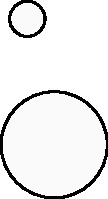
\includegraphics[width=0.10\textwidth]
{gesamttex/edit_VIII-4/images/LH_37_03_115-116_d_116v.pdf}%
\edcaption[0.25em]{%
\lbrack\textit{Fig.\:1}\rbrack%
}%
\end{edfigure}%
\newpage%
\pstart%
\edlabel{LH_37_03_115-116_116v_aestusmaris-1}%
Quousque autem pressionis hujus vis%
\indexS{vis pressionis aeris subtilis}%
\indexS{pressio aeris subtilis}
se extendat
ignotum
\edtext{%
est,
crediderim maximam esse 
et fortasse aeris tenuissimi sphaeram%
\indexS{sphaera aeris tenuis}
ad ipsam usque lunam%
\indexS{luna}
et ultra assurgere.%
}{%
\lemma{est,}%
\Bfootnote{%
\textit{(1)}~credidi sp %
\textit{(2)}~crediderim %
\bars{esse multo \textit{streicht Hrsg.}} maximam esse %
\textit{(a)}~quonam aeris hujus %
\textit{(b)}~aerisque hujus sphaeram forte sese %
\textit{(c)}~et fortasse %
\lbrack...\rbrack\ et ultra %
\textit{(aa)}~extendi %
\textit{(bb)}~assurgere.%
~\textit{L}%
}}
Et posito Lunam%
\indexS{luna}
gravitate carere%
\indexS{gravitas lunae}
neque ad terram nostram tendere,%
\indexS{terra}
sustinebit ipsa cylindrum aeris ultra-lunaris%
\indexS{aer ultra-lunaris}%
\indexS{cylinder aeris superimminens lunae}
sibi superimminentem %
et quominus terram premat prohibebit.%
\indexS{cylinder aeris premens terram}%
\indexS{terra}
Unde mare lunae subjectum%
\indexS{mare subjectum lunae}
\edtext{%
minus quam reliquus oceanus premetur%
\indexS{oceanus}
et ideo%
}{%
\lemma{minus}%
\Bfootnote{%
\textit{(1)}~pressum quam %
\textit{(a)}~ambiens %
\textit{(b)}~reliquus oceanus %
\textit{(2)}~quam reliquus %
\lbrack...\rbrack\ et ideo%
~\textit{L}%
}}
cum lunam in Meridiano%
\indexS{luna in meridiano}%
\indexS{meridianus}
habebit intumescet.%
\indexS{mare intumescens sub luna}
Sed haec conjectura%
\indexS{conjectura examinanda}
diligentius
\edtext{%
alias%
}{%
\lemma{alias}%
\Bfootnote{%
\textit{erg.}%
~\textit{L}%
}}
examinanda est;
explicandumque
quomodo omnia loca%
\indexS{locus sub meridiano lunae}
sub meridiano lunae posita
\edtext{%
simul afficiantur.%
}{%
\lemma{simul}%
\Bfootnote{%
\bars{tantum \textit{gestr.}} afficiantur.%
~\textit{L}%
}}%
\edlabel{LH_37_03_115-116_116v_aestusmaris-2}
\edlabel{LH_37_03_115-116_116v_schedapeculiaris-1}%
De quo
\edtext{%
scheda peculiari.%
\indexS{scheda peculiaris}%
\edlabel{LH_37_03_115-116_116v_schedapeculiaris-2}%
}{%
\lemma{scheda peculiari}%
\Cfootnote{%
Wohl Anspielung auf die (voraussichtlich in einem späteren Band von \textit{LSB} VIII zu edierende) Aufzeichnung \textit{De aestu maris ratio nova plane singularis; accessit suspicio de declinatione magnetica deque annulo lunari fluido circa Terram, ut est solidus circa Saturnum} (LH XXXV\;13,\;3 Bl.\;194). %
Das Manuskript ist von Leibniz eigenhändig auf April 1683 datiert.
}}
\pend%
\pstart%
Tantum
\pend%
\vspace*{1.5em}%
\pstart%
\noindent%
\centering%
*     *     *
\pend%
\vspace{2.75em}%
\selectlanguage{german}%
\frenchspacing%
\footnotesize%
\pstart%
\noindent%
\textls{Ausführliche Datierungsgründe:}%
\pagelabel{60205_dat}
Im Mittelpunkt der undatierten Aufzeichnung N.\;\ref{60205} \textit{De nova pressione aeris subtilioris etiam intra locum aere communi exhaustum deprehensa, et in aere libero pressionem a cylindro aeris crassi ortam longe superante} steht Leibnizens Annahme eines besonderen Fluidums, welches sich als "dünnere Luft" mit der wahrnehmbaren Luft vermische, durchdrigender als diese letztere sei und durch seinen Druck Phänomene hervorbringe, die unter bloßer Berücksichtigung des gewöhnlichen Luftdrucks unerklärbar wären (wie etwa Adhäsion im Vakuum).
Die Datierung der Aufzeichnung N.\;\ref{60205} ergibt sich aus folgenden Beobachtungen:
\pend%
\pstart%
(1)
Am Ende der Aufzeichnung N.\;\ref{60205} \textit{De nova pressione aeris subtilioris} gibt Leibniz, im Anschluss an die Frage nach der Höhe der die Erde um\-fassenden Sphäre "dünnerer Luft", eine skizzenhafte Erklärung des Phänomens der Gezeiten ab, der zufolge die Erhöhung des Meeresspiegels in der Phase der Flut von einer Verkürzung der Luftsäule durch den %
Mond herrühren soll (vgl. oben, \refpassage{LH_37_03_115-116_116v_aestusmaris-1}{LH_37_03_115-116_116v_aestusmaris-2}).
Daraufhin kundigt er an, die dargelegte Mutmaßung in einer \textit{scheda peculiaris} ausführlich erörten zu wollen (vgl. oben, \refpassage{LH_37_03_115-116_116v_schedapeculiaris-1}{LH_37_03_115-116_116v_schedapeculiaris-2}).
Nach heutigem Wissenstand finden sich im Nachlass zwei (voraussichtlich in einem späteren Band von \textit{LSB} VIII zu edierende) handschriftliche Aufzeichnungen, in denen sich Leibniz ausführlich um eine Erklärung der Gezeiten bemüht:
das Manuskript LH XXXV\;13,\;3 Bl.\;194, %
das die Überschrift
\ledpb%
\textit{De aestu maris ratio nova plane singularis; accessit suspicio de declinatione magnetica deque annulo lunari fluido circa Terram,
ut est solidus circa Saturnum} aufweist und von Leibniz eigenhändig auf April 1683 datiert ist;
sowie das titellose und undatierte Manuskript LH\;XXXVII\;4 Bl.\;109. %
In diesem letzteren findet der am Ende der Aufzeichnung N.\;\ref{60205} umrissene Erklärungsansatz keine Erwähnung.
Anders verhält es sich in der Aufzeichnung \textit{De aestu maris}: %
Dort wird gegen Ende des Textes (%
Bl.\;194\,v\textsuperscript{o}) -- unter der zusätzlichen Annahme eines rotierenden magnetischen Ringes, der den jeweiligen vom Mond besetzten Meridian umkreisen soll -- ein ähnlicher Erklärungsansatz dargelegt wie in N.\;\ref{60205}.
Dies rechtfertigt die Annahme, dass \textit{De aestu maris} die am Ende von N.\;\ref{60205} angekündigte \textit{scheda peculiaris} sein dürfte.
Eine im Kopf dieses Manuskriptes %
(Bl.\;194\,r\textsuperscript{o}) nachträglich hinzugefügte Randbemerkung -- \textit{Annulus, credo, inanis nec necessarius, vide aliam schedam} -- dürfte auf die titellose Aufzeichnung LH XXXVII\;4 Bl.\;109 %
hinweisen und somit zeigen, dass diese letztere erst nach \textit{De aestu maris} verfasst wurde.
Hieraus folgt, dass \textit{April 1683} als Terminus ante quem der Datierung von N.\;\ref{60205} anzusehen ist.
\pend%
\pstart%
(2)
Zur Bekräftigung dieser Feststellung gilt es zu beachten, dass in der Aufzeichnung N.\;\ref{60205} Jacob Bernoullis \textit{Dissertatio de gravitate aetheris} (Amsterdam 1683)\cite{01403} nicht erwähnt wird, obwohl sie thematisch durchaus relevant gewesen wäre:
Ähnlich wie Leibniz fasst Bernoulli\indexN{\textls{Bernoulli}, Jacob 1655\textendash1705} dort den Äther als nicht sinnenfälliges, aber mit Schwere versehenes Fluidum an, das physikalische Phänomene erklären soll, die der Druck der wahrnehmbaren Luft nicht zu erklären vermag.
(In der späteren Aufzeichnung N.\;\ref{41212} \textit{De aestimatione virium quas per aeris compressionem acquirere licet} wird hingegen ausdrücklich auf die \textit{Dissertatio de gravitate aetheris}\cite{01403} verwiesen; vgl. \refpassage{LH_35_09_25_001-002+004-005_005r_Bernoulli-1}{LH_35_09_25_001-002+004-005_005r_Bernoulli-2} im vorliegenden Band.)
Demgemäß ist zu vermuten, dass die Aufzeichnung N.\;\ref{60205} vor Leibnizens Lektüre von Bernoullis\indexN{\textls{Bernoulli}, Jacob 1655\textendash1705} Abhandlung entstand.
Leibniz hat diese letztere wohl nicht vor deren anonymer Rezension\cite{01406} im Märzheft 1683 der \textit{Acta eruditorum}\cite{01023} (S.\;106\textendash112) gekannt; gelesen hat er sie aber wahrscheinlich erst später. %
Das Buch war nämlich auf der Frankfurter\indexO{Frankfurt am Main} Michaelis-Messe 1682 (\textit{Catalogus universalis}, Bl.\;\bracks{D4\,r\textsuperscript{o}})\cite{02596} angekündikgt und auf der Leipziger\indexO{Leipzig} Ostermesse 1683 (\textit{Catalogus universalis}, Bl.\;B3\,v\textsuperscript{o})\cite{02597} ausgestellt worden, weshalb es frühestens ab dem Frühjahr 1683 auf dem Buchmarkt erhältlich gewesen sein dürfte (in beiden Katalogen ist der Titel auch ungenau angegeben: wohl das Zeichen für eine späte Auslieferung).
Im Briefwechsel wird die Abhandlung zum ersten und bisher einzigen Mal erst nach Leibnizens Italienreise\indexO{Italien} erwähnt, nämlich in seinem Brief an Jacob Bernoulli\indexN{\textls{Bernoulli}, Jacob 1655\textendash1705} vom 24.\;September/4.\;Oktober 1690; vgl. \textit{LSB} III,\;4 N.\;279, S.\;573.24\,f.\cite{01260} %
Leibniz dürfte somit erst etliche Zeit nach dem Erscheinen der anonymen Rezension\cite{01406} %
imstande gewesen sein, Bernoullis\indexN{\textls{Bernoulli}, Jacob 1655\textendash1705} \textit{Dissertatio de gravitate aetheris}\cite{01403} in die Hände zu bekommen, jedenfalls nicht vor April 1683.
\pend%
\pstart%
(3)
Für die Bestimmung des Terminus post quem der Datierung von N.\;\ref{60205} ist zunächst zu beachten, dass das im Textträger von N.\;\ref{60205} anzutreffende Harzer Wasserzeichen im Leibniz-Nachlass nicht vor 1679 belegt ist und überhaupt nicht vor 1678 verwendet wurde. %
Das gleiche Wasserzeichen ist zudem im Träger von \textit{De aestu maris} sowie in LH\;XXXVII\;4 Bl.\;109 (siehe oben) anzutreffen.
Daher ist anzunehmen, dass die Aufzeichnung N.\;\ref{60205} zwischen 1679 und April 1683 -- wahrscheinlich aber eher gegen Ende dieser Zeitspanne -- entstand.
Leibniz hielt sich ohnehin erst ab dem Herbst 1680 regelmäßig im Harz\indexO{Harz} auf.
Somit dürfte N.\;\ref{60205} nicht vor dem Herbst 1680 abgefasst worden sein.
\pend%
\pstart%
(4)
Leinbiz erwähnt in N.\;\ref{60205} (\refpassage{LH_37_03_115-116_115r_deVolder-1}{LH_37_03_115-116_115v_deVolder-2}) ein Experiment zur Vermessung der Adhäsionskraft zweier in der Luft hängender Marmorplatten, das der kartesianische Physiker und Philosoph Burchard de Volder\indexN{\textls{Volder} (Volter, Wolder), Burchard (Burcher) de 1643\textendash1709} im März 1676 in Leiden\indexO{Leiden} durchgefürt hatte.
Von diesem Experiment hatte Leibniz aus einem ausführlichen Bericht erfahren können, welcher in der von Philipp Lohmeier\indexN{\textls{Lohmeier} (Lohmeierus, Lomeierus), Philipp 1648\textendash1680} betreuten und von Johann Pestel\indexN{\textls{Pestel}, Johann, 1678 in Rinteln promoviert} eingereichten Dissertation \textit{Exercitationum physicarum de paradoxi gravitatis et levitatis prima}, paradoxon I, §\;IX (Rinteln 1678, S.\;32--34)\cite{01429} zu lesen war.
(Das bei der GWLB Hannover unter der Signatur M-A 262 aufbewarte Exemplar weist Gerbrauchsspuren, die wahrscheinlich auf Leiniz zürückgehen.)
Das Experiment hatte Lohmeier\indexN{\textls{Lohmeier} (Lohmeierus, Lomeierus), Philipp 1648\textendash1680} aber auch in seinem Brief an Leibniz vom 23.\:August\;/\;2.\:September 1679 geschildert (\textit{LSB} III,\;2 N.\;336, S.\;817.16--20).\cite{01425}
Über einen ähnlichen von de Volder\indexN{\textls{Volder} (Volter, Wolder), Burchard (Burcher) de 1643\textendash1709} angestellten Versuch hatte ferner die anonyme Bemerkung "Experience faite à Leyden" im \textit{Journal des sçavans} vom 17.\;April 1679 (S.\;107\,f.)\cite{02524} erzählt,
worauf Ehrenfried Walther von Tschirnhaus\indexN{\textls{Tschirnhaus} (H. v. Tch., H. v. Tsch.), Ehrenfried Walther v. 1651\textendash1708} in seinem Brief an Leibniz vom 11.\;September 1682 flüchtig anspielt (\textit{LSB} III,\;3 N.\;399, S.\;711.8\,f.).\cite{02525}
Kannte Leibniz, wie es plausibel erscheint, De Volders\indexN{\textls{Volder} (Volter, Wolder), Burchard (Burcher) de 1643\textendash1709} Experiment mit den Marmorplatten vornehmlich aus Lohmeiers\indexN{\textls{Lohmeier} (Lohmeierus, Lomeierus), Philipp 1648\textendash1680} \textit{Exercitationum physicarum de paradoxi gravitatis et levitatis prima},\cite{01429} so ist zu vermuten, dass die Erwähnung des Experiments in N.\;\ref{60205} (\refpassage{LH_37_03_115-116_115r_deVolder-1}{LH_37_03_115-116_115v_deVolder-2}) wahrscheinlich erst einige Zeit nach Leibnizens Lektüre der Dissertation\cite{01429} erfolgt sein sollte.
Denn zwar wiedergibt Leibniz korrekt die Details des Verfahrens (hauptsächlich die Verwendung von Fett zum Abdichten), kann sich aber nicht mehr an das Gewicht erinnern, dessen es nach de Volders\indexN{\textls{Volder} (Volter, Wolder), Burchard (Burcher) de 1643\textendash1709} Angabe zum Abtrennen der Platten bedurft hatte.
Wenn man bedenkt, dass Leibniz die laut Titelblatt im August 1678 an der Universität zu Rinteln\indexO{Rinteln} verteidigte Dissertation frühestens einige Monaten nach deren Erscheinen lesen konnte (möglicherweise nach dem Empfangen von Lohmeiers\indexN{\textls{Lohmeier} (Lohmeierus, Lomeierus), Philipp 1648\textendash1680} Brief\cite{01425} vom 23.\:August\;/\;2.\:September 1679), 
dann dürfte die besagte Erwähnung in N.\;\ref{60205} (\refpassage{LH_37_03_115-116_115r_deVolder-1}{LH_37_03_115-116_115v_deVolder-2}) erst im Laufe der frühen 1680er Jahren verfasst worden sein.
\pend%
\pstart%
(5)
Es gilt schließlich zu bemerken, dass auch in weiteren Texten der frühen 1680er Jahre Leibniz die Hypothese eines luftähnlichen, aber unermeßlich viel dünneren umgebenden Fluidums aufgestellt hatte, um physikalische Phänomene zu erklären, die unter bloßer Berücksichtigung der wahrnehmbaren Luft unerklärbar wären.
Dies ist besonders deutlich in dem auf die Zeitspanne zwischen Januar und März/April 1683 datierbaren Entwurf \textit{Explicatio mechanica elastri, seu causa cur corpora per vim tensa spopnte restitui videantur}\cite{01437} der Fall, in dem Leibniz das besagte umgebende Fluidum in Anspruch nimmt, um Grundeigenschaften makroskopischer Körper wie Elastizit und Kohäsion verständlich zu machen (vgl. \textit{LSB} VIII,\;3 N.\;14\textsubscript{3}, bes. S.\;211.16--212.5).
Demnach ist plausibel, dass auch die Aufzeichnung N.\;\ref{60205} im Zusammenhang mit einem Text wie \textit{Explicatio mechanica elastri} und in einem gemeinsamen Zeitraum verfasst wurde, d.\,h. zwischen Januar und April 1683.
Eine frühere Entstehung (wohl ab dem Herbst 1680) ist jedoch nicht auszuschließen.
\pend%
\pstart%
Aus den angegebenen Gründen ergibt sich als Gesamtdatierung der Aufzeichnung N.\;\ref{60205} \textit{De nova pressione aeris subtilioris} %
die Zeitspanne vom Herbst 1680 bis zum April 1683.
Vor 1680 ist sie unwahrscheinlich entstanden;
vielmehr dürfte sie gegen Ende der angegebenen Zeitspanne niedergeschrieben worden sein.
\pend%
\selectlanguage{latin}%
\frenchspacing%
\newpage%
